\section{Literature Review}
\begin{itemize}
    \item explain what a neural network is in general
    \item brief summary on how the learning works (backpropagation)
\end{itemize}

\subsection{Types of Deep Learning Methods}
\begin{itemize}
    \item compare training methods for deep learning (supervised, unsupervised, reinforcement learning)
    \item emphasize requirements and advantages of the different methods
    \item raise ideas how the methods can be used throughout the thesis
\end{itemize}

\subsection{Convolutional Neural Networks}
One subclass of neural networks is called \emph{Convolutional Neural Network} (CNN) ~\cite[p.~359]{praxiseinstieg_ml17}. These types of networks show great results on data with a grid-like topology. Thus, they are often used for processing of image or video data. In traditional neural networks the layers are often densely connected, meaning every neuron of one layer is connected to every neuron in the next layer. For grid-like data this is not very efficient, because cells close to each other are often more likely to be correlated. Instead of dense connections, CNNs use operations called \emph{convolution} and \emph{pooling}, which allow to take spatial properties of the input data into account. The following sections explain the commonly used operations in CNNs.

\subsubsection{Convolution}
% TODO: be more precise with input/output of neurons
\emph{Convolution} is a mathematical operation that uses weighted point-by-point multiplication of two matrices resulting in a scalar value. The concept is shown in figure~\ref{fig:convolution}. The notation $n_{k,~i,~j}$ represents a neuron at row~$i$ and column~$j$ in layer~$k$. For a convolutional layer, neuron $n_{k,~i,~j}$ is connected to all neurons $n_{k-1,~i,~j}$ to $n_{k-1,~i + f_w -1,~j + f_h -1}$. The neurons in layer~$k-1$ are therefore called receptive field of $n_{k,~i,~j}$ with a kernel width of $f_w$ and kernel height of $f_h$.~\cite[p.~361 f]{praxiseinstieg_ml17}

% TODO replace image with proper illustration
\begin{figure}[h]
    \centering
    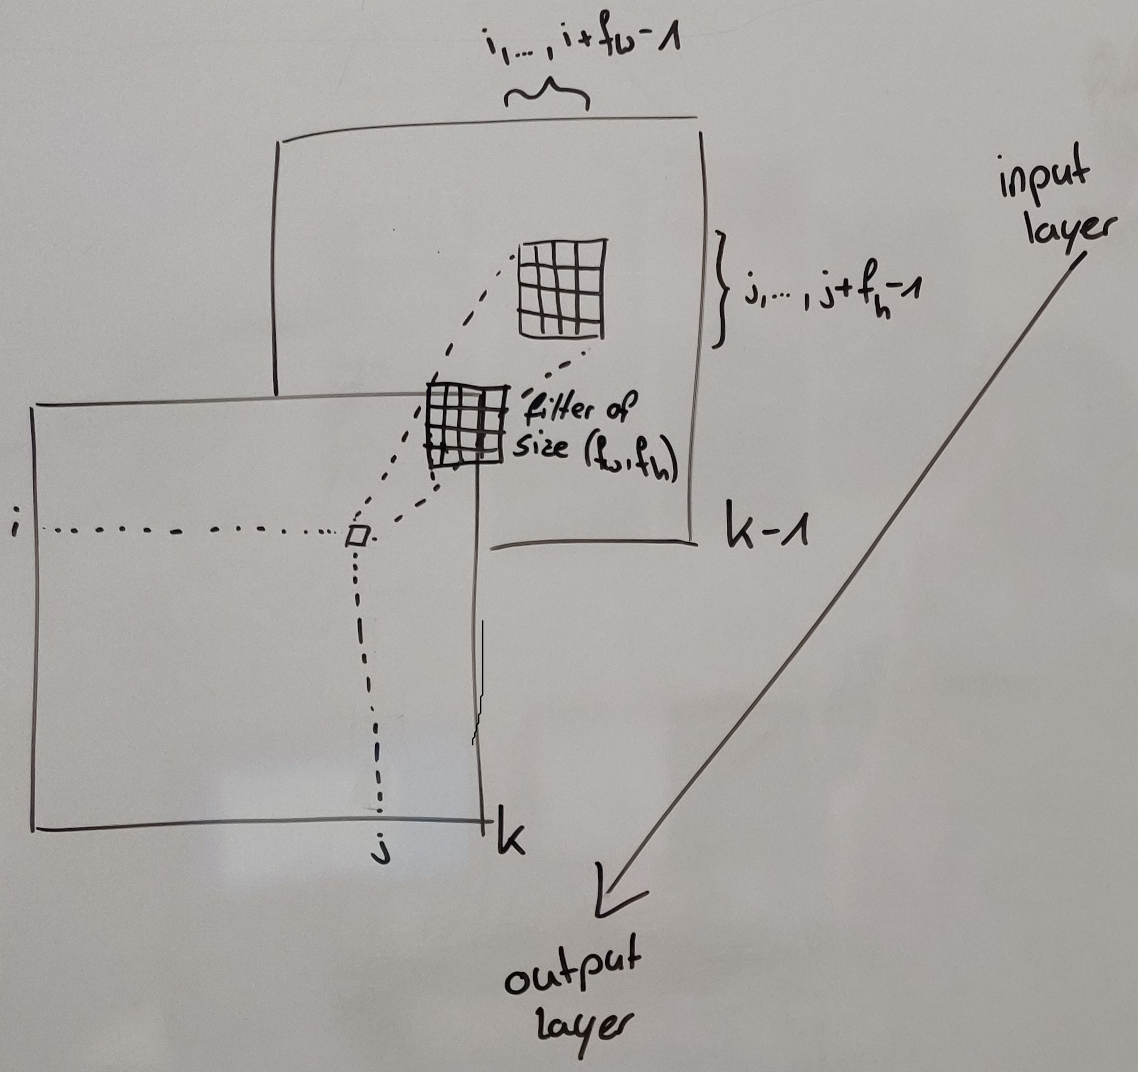
\includegraphics[width=0.6\textwidth]{images/convolution_template}
    \caption{Receptive field of a convolution operation}
    \label{fig:convolution}
\end{figure}

There are different ways to handle the edges of the grid. If no special action is taken, the output layer will be smaller in terms of edge length. For this reason \emph{zero padding} is often used to enlarge the input layer before convolution is performed. With an appropriate padding it is possible to preserve the width and height of the layer. Another parameter that affect the size of the output layer is called \emph{stride}, that controls the distance between to neighbouring receptive fields.~\cite[p.~361]{praxiseinstieg_ml17}

The trainable parameters in a convolution layer are the weights and biases used for the matrix multiplication introduced earlier. One specific set of weights and biases is called a \emph{filter}. It is responsible for detecting one single feature of the input layer. The output of a filter is thus referred to as \emph{feature map}. To inspect multiple features of the input, a convolution layer usually consists of multiple filters that are trained and calculated independently. In the end, the output of a convolution layer are multiple feature maps, each highlighting one single feature of the input.~\cite[p.~363 f]{praxiseinstieg_ml17}

As stated by Goodfellow et al.\ in~\cite{DLbook16} the convolution operation has some properties that are highly valuable to build an efficient and powerful neural network. Compared to traditional neural networks, convolution layers have only few connections between to subsequent layers. This is because the kernel is much smaller than the input. Especially for images, which can have millions of pixels, this helps to reduce the number of parameters to train.  Furthermore, the convolution reuses the same parameters for an entire feature map. Besides increasing the statistical efficiency of the model, it also makes the operation equivariant to translation in the input.

% TODO: explain the above section in more detail?
\begin{comment}
    \cite{DLbook16}
    330: NN use only matrix multiplication. meaning every output unit of one layer interacts with the all input units of the next layer. convolution leverages sparse interactions. for example images can have millions of pixels, but to detect edges it is enough to only look at a few pixels at a time. thus we can have a kernel smaller than the image size resulting in fewer parameters. This reduces memory requirements of the model and increases statistical efficiency.

    331, 333: another advantage is parameter sharing. with matrix multiplication you usually have a weight matrix, where each value is used only once. convolution operation uses parameter sharing, because one kernel is applied multiple times on the same image. and since kernel is smaller than image, it again reduces number of parameters by a significant amount.

    334f: due to parameter sharing, convolution operation is equivariant to translation. Meaning, if you move parts of the input convolution will still give you the same output, just with the moved detection. This is especially helpful for working with images, as object might be in different locations of the image, but should still be realized.
\end{comment}

\subsubsection{Pooling}
Unlike convolution, which is used to extract features from the input, \emph{pooling} removes information from the data to reduce the number of parameters and also to prevent overfitting. The procedure of pooling is similar to convolution. However, it does not use matrix multiplication but instead performs a predefined mathematical function on the input matrix. While any function can be used for the pooling operation, most of the times it is the $\max$ function. Thus, it reduces the available information but still keeps the most important activations.~\cite[p.~369 f]{praxiseinstieg_ml17}

Because the function to use is predefined, pooling layers do not contain any trainable parameters. But still they are configurable with the same hyperparameters as convolution layers, namely kernel size, stride and padding. In addition, you can not only do pooling along the two axis of the input, but also along the third axis, which are the feature maps.~\cite[p.~370]{praxiseinstieg_ml17}

% TODO replace image with proper illustration
\begin{figure}[h]
    \centering
    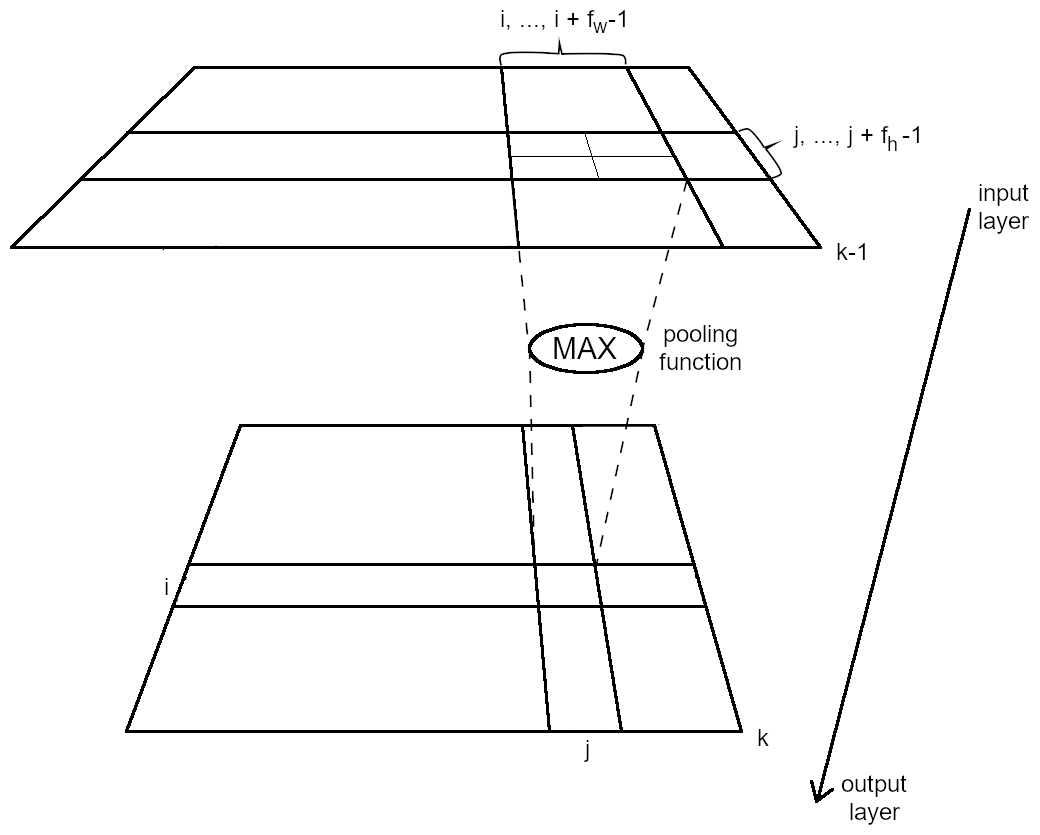
\includegraphics[width=0.6\textwidth]{images/maxpool_template}
    \caption{Max pooling}
    \label{fig:pooling}
\end{figure}

\subsubsection{Other Important Concepts}
\begin{itemize}
    \item Batch Normalization
    \item ReLU Activation
\end{itemize}

\subsection{Reference Architectures}
\begin{itemize}
    \item make clear why it is convenient to use reference architectures
\end{itemize}

\subsubsection{U-Net Architecture}
%TODO: go more into detail on the training and the results they achieved
In 2015, Ronneberger et al.\ introduced an architecture called \emph{U-Net} which they recommended for binary segmentation of biomedical images~\cite{unet15}. As can be seen in figure~\ref{fig:unet_architecture}, this name derives from the U-shape of the network model. It consists of a contracting path in the beginning, in which convolution and pooling layers are used to condense the input. The second half forms an expansive part, that uses convolution and upsampling layers to go back to the scale of the original image. Note that the outputs of the convolution layers in the contracting path are cropped and then concatenated to the input layers with the corresponding size in the expansive path. By doing that, the expansive layers still retain enough information from the original input to deliver a precise segmentation.

\begin{figure}[h]
    \centering
    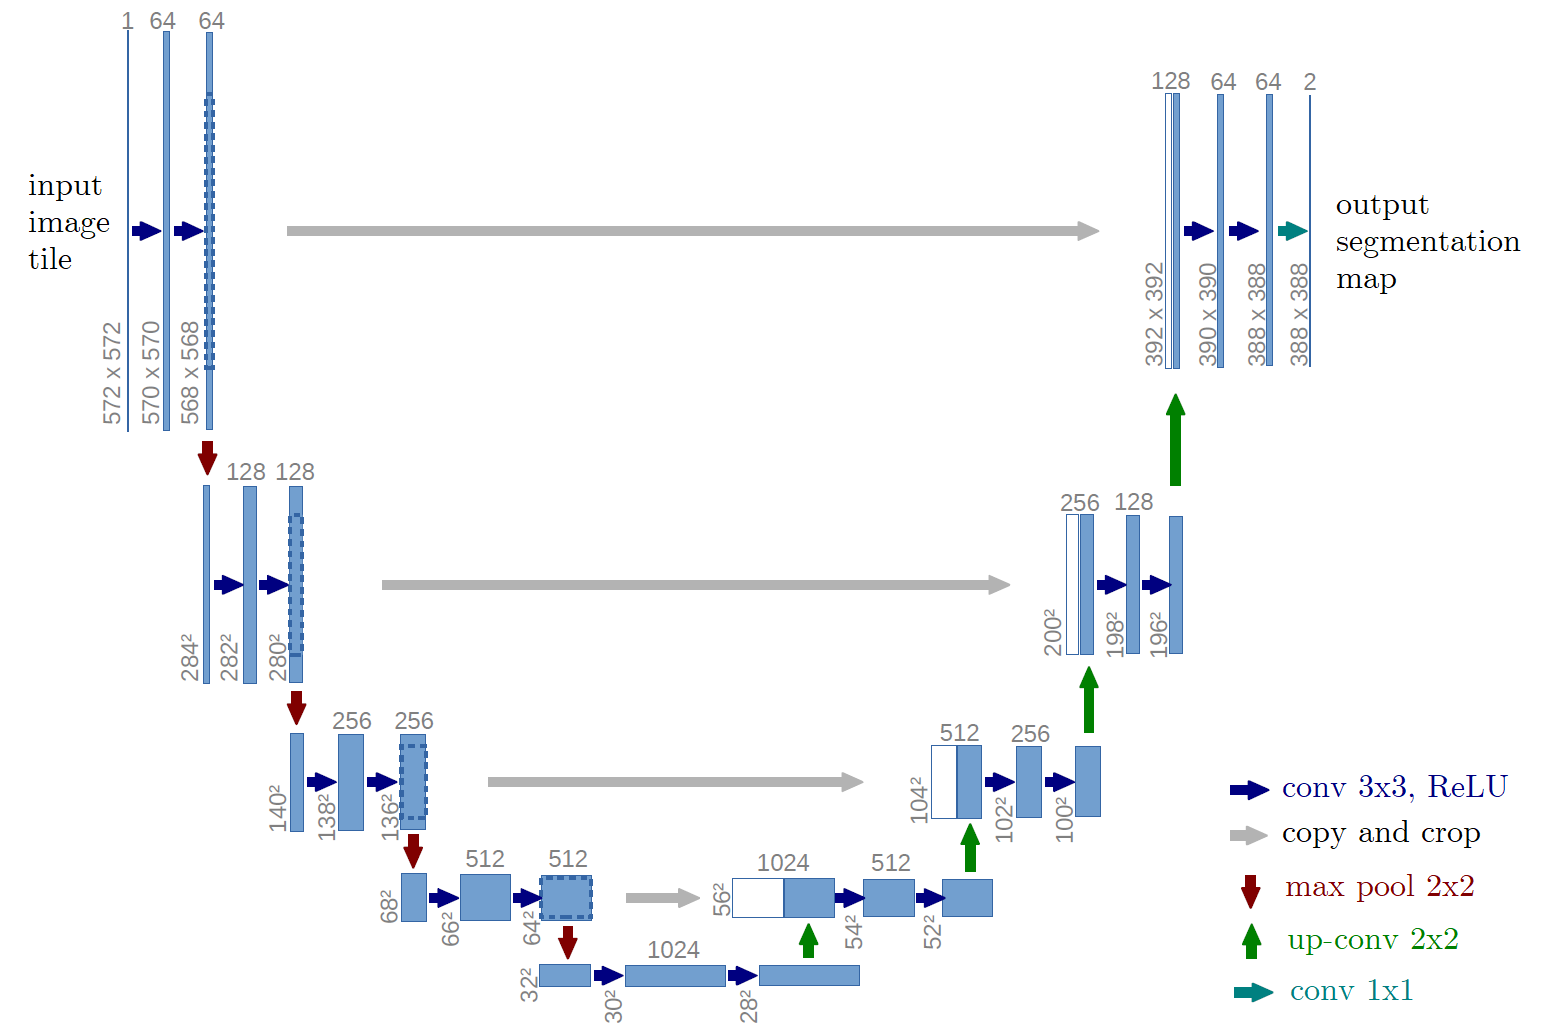
\includegraphics[width=0.9\textwidth]{images/u-net-architecture}
    \caption{U-Net Architecture \cite{unet15}}
    \label{fig:unet_architecture}
\end{figure}

The U-Net architecture contains neither fully connected layers nor do they use padding for the edges. Thus, the segmentation map has a lower resolution that the original image, because it only contains pixels for which the full context is available. By using a tiling strategy with overlapping tiles, this approach can produce seamless segmentation maps for input images of arbitrary size. For the edges of the input image, Ronneberger et al.\ suggest a mirroring strategy to extrapolate the missing context.~\cite{unet15}


\subsubsection{DenseNet Architecture}
As the depth of CNN architectures tends to increase, a new challenge arose regarding the training of those networks. Since the hidden layer can be very far away from the input and output layers, the values and gradients passed between the layers can get lost on the way. In an attempt to solve this, Huang et al.\ came up with the idea to directly connect all layers with matching feature map sizes. They published their architecture under the name \emph{DenseNet} in~\cite{densenet18}.

Huang et al.\ see the values passed between layers as a state. To access the state of one of the early layers in the network with a subsequent layer, all the layers in between have to pass the state unchanged, thus creating redundancy. With the DenseNet architecture, the state of all previous layers is explicitly passed to subsequent layers. This means, the network now differentiates between information that originates from an earlier layer and new information found in the current layer. It allows to keep the convolution layers narrow, because each layer only adds information, but never changes information that was previously acquired. This concept leads to having fewer trainable parameters and an improved flow of gradients, which both reduce the effort for training the network.~\cite{densenet18}

\begin{figure}[h]
    \centering
    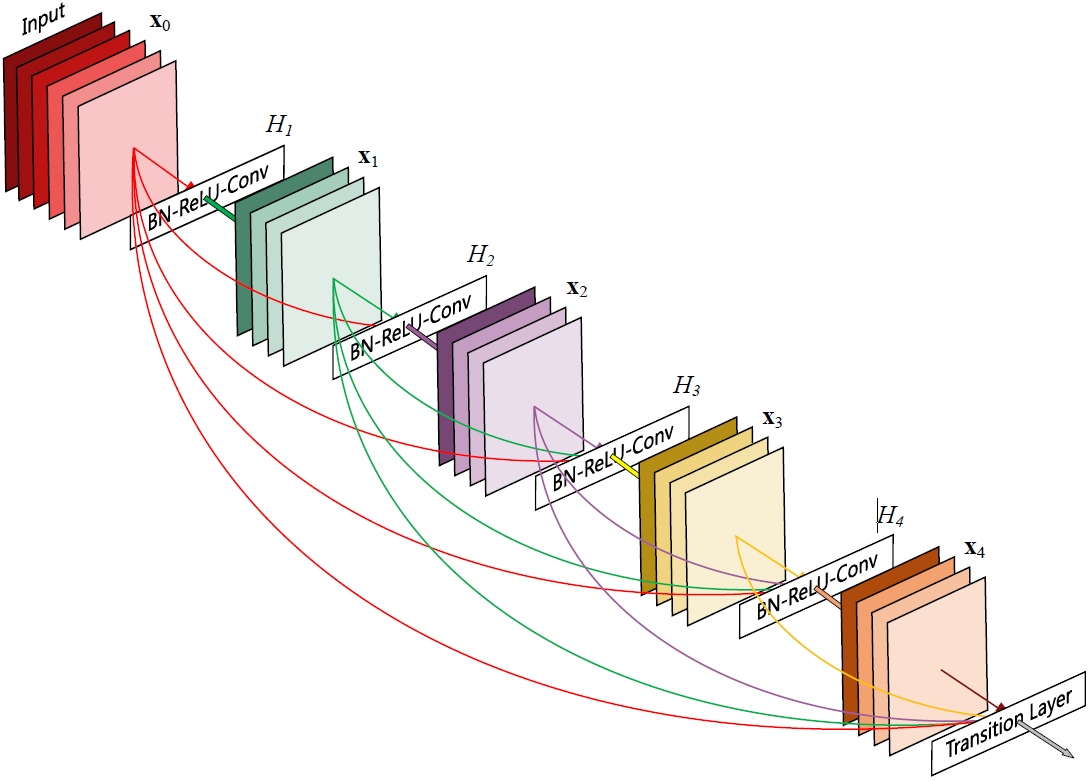
\includegraphics[width=0.7\textwidth]{images/dense-net-architecture}
    \caption{Densely Connected Convolutional Architecture \cite{densenet18}}
    \label{fig:densenet_architecture}
\end{figure}

To add the connections between the layers, the authors simply concatenate the feature maps. Thus, it is not possible to connect layers which feature maps are of different size. To still be able to use pooling layers to condense the information in the network, the authors introduce a component called \emph{dense block} as illustrated in figure~\ref{fig:densenet_architecture}. Inside of a dense block, they apply dense connections between the convolution layers. In between two consecutive dense blocks, there is a \emph{transition layer}, which is formed by a convolution and an average pooling layer. Ultimately, the overall architecture of a DenseNet consists of several independent dense blocks separated by transition layers, eventually concluded by a fully-connected layer.

\subsection{Architecture Comparison}
Interesting for architecture comparison: \cite{imseg_architecures}

\begin{itemize}
    \item point out the common characteristics and differences of the architectures
    \item compare use cases of the architectures and how they perform on them
\end{itemize}

\newpage